
\documentclass[conference]{IEEEtran}

\usepackage[utf8]{inputenc}
\usepackage[T1]{fontenc}
\usepackage[english]{babel}
\addto\captionsenglish{\renewcommand{\figurename}{Fig.}}
\usepackage{float}
\usepackage{graphicx}
\usepackage{amsmath, amssymb}
\usepackage{booktabs}
\usepackage{array}
\usepackage{natbib}
\usepackage{hyperref}
\usepackage{tikz}
\usepackage{xcolor}
\usetikzlibrary{arrows.meta, positioning, fit, backgrounds}
\definecolor{thesisBlue}{RGB}{225,234,245}
\definecolor{thesisBlueD}{RGB}{46,84,130}

\hypersetup{
  colorlinks=false,
  pdfborder={0 0 1},
  linkbordercolor=red,
  citebordercolor=green,
  urlbordercolor=blue
}

\begin{document}

\title{Anomaly Detection for Healthcare Applications}

\author{
\IEEEauthorblockN{Ceren Yıldız}
\IEEEauthorblockA{
\textit{Department of Statistics}\\
Eskişehir, Türkiye\\
cerenyildiiiz26@gmail.com}
}

\maketitle

\renewcommand{\abstractname}{Özetçe}
\begin{abstract}
Bu çalışma, sağlık uygulamalarında anomali tespiti problemini ele almakta ve biyomedikal zaman serisi verilerindeki anormal örüntülerin belirlenmesine odaklanmaktadır. Normal ile anormal örüntüleri ayırt etmek amacıyla derin öğrenme tabanlı yaklaşımlar incelenmekte; temsili bir uygulama olarak EKG sinyalleri üzerinde 1D-CNN ve LSTM mimarileri değerlendirilmektedir.
\end{abstract}

\renewcommand{\IEEEkeywordsname}{Anahtar Kelimeler}
\begin{IEEEkeywords}
anomali tespiti, sağlık uygulamaları, EKG sinyalleri, zaman serisi, derin öğrenme
\end{IEEEkeywords}

\renewcommand{\abstractname}{Abstract}
\begin{abstract}
This study addresses anomaly detection in healthcare applications, focusing on abnormal patterns in biomedical time-series data. We examine deep learning approaches for distinguishing normal from anomalous patterns and, as a representative application, evaluate 1D-CNN and LSTM architectures on ECG signals to support the early identification of abnormal cardiac conditions.

Code: \url{https://github.com/cerenyildiiz/ecg5000-anomaly-detection-time-series}
\end{abstract}

\renewcommand{\IEEEkeywordsname}{Keywords}
\begin{IEEEkeywords}
anomaly detection, healthcare applications, ECG signals, time series, deep learning
\end{IEEEkeywords}

\section{Introduction}

Anomaly detection is the task of finding patterns in data that do not match what is expected. In healthcare, such patterns can be as critical as an irregular heartbeat, yet reliably spotting them across large amounts of data is slow and error-prone for a human observer.

Machine learning methods have been applied to early diagnosis, anomaly detection and failure prediction in many domains \citep{sarker2021}. This study focuses on ECG signals, which record the heart's electrical activity. A healthy heart produces a fairly regular waveform, so deviations can indicate a cardiac condition. We explore how a 1D convolutional neural network (1D-CNN) and an LSTM autoencoder can detect abnormal heartbeats directly from raw signals, without manual feature engineering. The workflow is summarized in Fig.~\ref{fig:workflow}.

\begin{figure}[H]
    \centering
    \resizebox{\columnwidth}{!}{%
    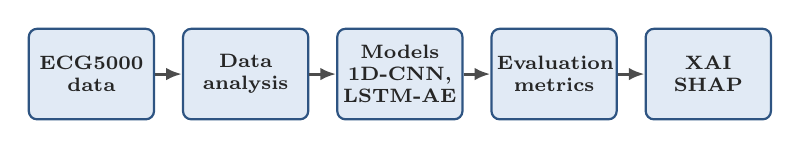
\begin{tikzpicture}[
        node distance=0.34cm,
        wbox/.style={draw=thesisBlueD, fill=thesisBlue, line width=0.8pt, rounded corners=3pt,
            text width=1.45cm, minimum height=1.15cm, align=center, inner sep=2pt,
            font=\scriptsize\bfseries, text=black!85},
        arr/.style={-{Latex[length=2mm,width=1.6mm]}, line width=1.1pt, black!70}
    ]
        \node[wbox]  (a) {ECG5000\\data};
        \node[wbox,  right=of a] (b) {Data\\analysis};
        \node[wbox,  right=of b] (c) {Models\\1D-CNN,\\LSTM-AE};
        \node[wbox, right=of c] (d) {Evaluation\\metrics};
        \node[wbox,  right=of d] (e) {XAI\\SHAP};
        \foreach \x/\y in {a/b, b/c, c/d, d/e} \draw[arr] (\x) -- (\y);
    \end{tikzpicture}%
    }
    \caption{Overall workflow of the study.}
    \label{fig:workflow}
\end{figure}

\section{Related Work}

ECG5000 is one of the most common benchmarks for ECG anomaly detection. Table~\ref{tab:related-work} summarizes representative studies.

Adegoke-Elijah et al.\ use an LSTM autoencoder and report 99.23\% accuracy and 98.00\% AUC \citep{adegoke2025}. Nayana and Vinay combine an LSTM autoencoder with SHAP to visualize the temporal segments behind an anomaly prediction, reaching 97.6\% accuracy and a 96.7\% F1-score \citep{nayana2026}. Alamr and Artoli propose an unsupervised transformer-encoder model validated on ECG5000 and MIT-BIH Arrhythmia \citep{alamr2023}. Shi and Jiang introduce LAVAE-Net, an LSTM-attention variational autoencoder trained only on normal heartbeats, with a 99.4\% F1-score \citep{shi2026}. Wu et al.\ use adaptive Toeplitz convolution kernels designed around the shape of ECG signals, improving accuracy and runtime \citep{wu2025}.

\begin{table}[H]
    \centering
    \caption{Representative studies on ECG5000 (results as reported by the authors; not directly comparable due to different evaluation protocols).}
    \label{tab:related-work}
    \scriptsize
    \setlength{\tabcolsep}{3pt}
    \begin{tabular}{>{\raggedright\arraybackslash}p{1.75cm}>{\raggedright\arraybackslash}p{2.05cm}>{\raggedright\arraybackslash}p{1.4cm}>{\raggedright\arraybackslash}p{2.15cm}}
        \toprule
        \textbf{Study} & \textbf{Model} & \textbf{Dataset} & \textbf{Reported result} \\
        \midrule
        Adegoke-Elijah et al.\ (2025) & LSTM autoencoder & ECG5000 & Acc.\ 99.23\%, AUC 98.00\% \\
        Nayana and Vinay (2026) & LSTM autoencoder + SHAP & ECG5000 & Acc.\ 97.6\%, F1 96.7\% \\
        Alamr and Artoli (2023) & Transformer encoder & ECG5000, MIT-BIH & Acc.\ 99\% (ECG5000), 89.5\% (MIT-BIH) \\
        Shi and Jiang (2026) & LSTM-attention VAE & ECG5000 & F1 99.4\% \\
        Wu et al.\ (2025) & Toeplitz convolution classifier & ECG5000 & Acc.\ above 99.6\% \\
        \bottomrule
    \end{tabular}
\end{table}

Most of these studies focus on detection performance, while only a few address interpretability. Here, a 1D-CNN serves as a baseline, an LSTM autoencoder is considered for reconstruction-based detection, and SHAP is planned for explaining decisions over the time dimension.

\section{1D Convolutional Neural Network}

Convolutional neural networks (CNNs) are among the most widely used deep learning architectures \citep{gharehbaghi2023}. A 1D-CNN slides learnable kernels over one-dimensional data such as time series. For an input $x$ of length $L$ with $C$ channels, the output of the $j$-th filter at position $t$ is
\begin{equation}
    y_j[t] = b_j + \sum_{c=1}^{C}\sum_{k=0}^{K-1} w_{j,c}[k]\; x_c[s\,t + k - p],
\end{equation}
where $K$ is the kernel size, $s$ the stride, $p$ the padding, $w_{j,c}$ the weights and $b_j$ the bias. The output length is
\begin{equation}
    L_{\text{out}} = \left\lfloor \frac{L + 2p - K}{s} \right\rfloor + 1 .
\end{equation}
For $L=140$, $K=8$, $s=2$ and $p=3$, this gives $L_{\text{out}}=70$, matching the $2\times70$ feature map in Fig.~\ref{fig:cnn-model}. After ReLU, $\mathrm{ReLU}(z)=\max(0,z)$, max pooling with kernel size 2 halves the length to 35. The flattened 70 features pass through two dense layers, and a softmax converts the final scores $z_k$ into class probabilities,
\begin{equation}
    \hat{y}_k = \frac{e^{z_k}}{\sum_{i} e^{z_i}} .
\end{equation}
The network minimizes the mean squared error over $N$ training samples,
\begin{equation}
    \mathcal{L} = \frac{1}{N}\sum_{n=1}^{N} \left\lVert \hat{\mathbf{y}}_n - \mathbf{y}_n \right\rVert_2^2 .
\end{equation}

\section{ECG5000 Dataset}

ECG5000 contains 5,000 heartbeats, each with 140 amplitude values and one class label; there are no missing values \citep{ferreira2022}. The original training and test files are combined into a single set. The five classes are: Normal (N), R-on-T Premature Ventricular Contraction (R-on-T PVC), Premature Ventricular Contraction (PVC), Supraventricular Premature or Ectopic Beat (SP) and Unclassified Beat (UB).

For anomaly detection, class 1 (Normal) is treated as normal and classes 2--5 as anomalous, giving 2,919 normal beats (58.4\%) and 2,081 anomalous beats (41.6\%). As Fig.~\ref{fig:class-distribution} shows, the binary problem is only moderately imbalanced, but the anomalous classes are strongly imbalanced (PVC: 96, SP: 194, UB: 24). A model ignoring the rare classes could therefore still reach a high overall accuracy.

\begin{figure}[H]
    \centering
    \includegraphics[width=\linewidth]{heartbeat_class_distribution.png}
    \caption{Class distribution of the ECG5000 dataset.}
    \label{fig:class-distribution}
\end{figure}

Fig.~\ref{fig:mean-ecg-by-class} shows the mean waveform of each class. The Normal class has a distinctive shape, with a pronounced peak of about 1.5 near time point 105 and a narrow variability band. The anomalous classes lose this structure: R-on-T PVC and PVC show a broad plateau instead of a sharp peak and end with a steep drop, SP follows a similar trend with a different amplitude, and UB has the widest band, probably because it is a mixed and very small class. These differences suggest the classes can be separated from the raw signal.

\begin{figure}[H]
    \centering
    \includegraphics[width=\linewidth]{mean_ecg_by_class.png}
    \caption{Mean ECG waveform of each class. Shaded areas show variability around the mean.}
    \label{fig:mean-ecg-by-class}
\end{figure}

\section{1D-CNN Model Training}

A single-layer 1D-CNN is trained on the 140-point signals with the Adam optimizer and MSE loss. The hyperparameters are given in Table~\ref{tab:hyperparameters} and the architecture in Fig.~\ref{fig:cnn-model}.

\begin{table}[H]
    \centering
    \caption{Hyperparameters of the 1D-CNN model.}
    \label{tab:hyperparameters}
    \begin{tabular}{ll}
        \toprule
        \textbf{Setting} & \textbf{Value} \\
        \midrule
        Model & Single-layer 1D-CNN \\
        Optimizer & Adam \\
        Learning rate & 0.001 \\
        Loss function & Mean squared error (MSE) \\
        Batch size & 32 \\
        Epochs & 10 \\
        \bottomrule
    \end{tabular}
\end{table}

\begin{figure}[H]
    \centering
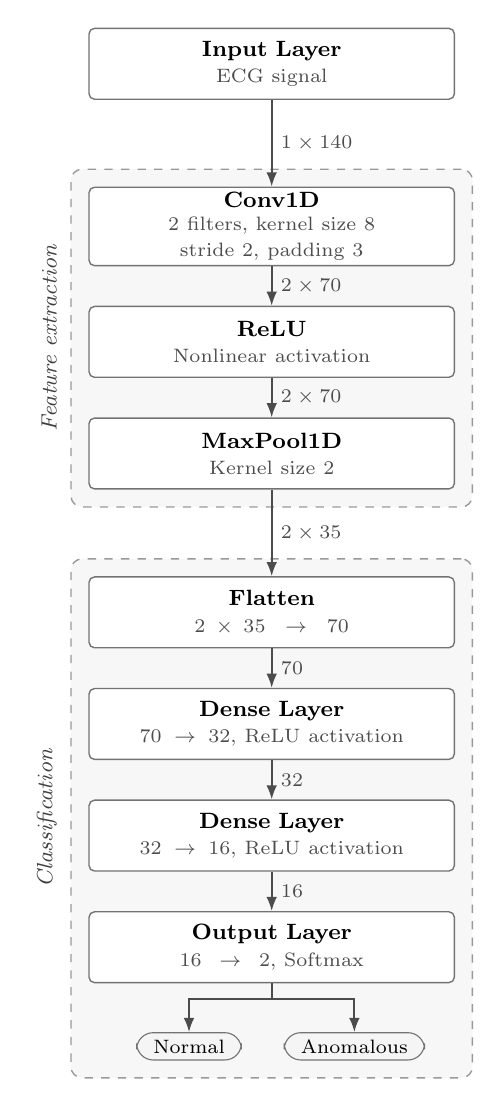
\begin{tikzpicture}[
    node distance=0.5cm,
    card/.style={draw=black!55, line width=0.5pt, rounded corners=2pt, fill=white,
        text width=4.5cm, align=center, minimum height=0.9cm, inner sep=2pt, font=\footnotesize},
    shp/.style={font=\scriptsize, text=black!70, anchor=west, inner sep=3pt},
    arr/.style={-{Latex[length=1.8mm]}, line width=0.7pt, black!70},
    tag/.style={draw=black!55, fill=gray!8, rounded corners=6pt, font=\scriptsize,
        inner xsep=6pt, inner ysep=2.5pt},
    stage/.style={draw=black!40, dashed, line width=0.5pt, rounded corners=4pt,
        fill=gray!6, inner sep=0.22cm}
]
    \node[card] (in) {\textbf{Input Layer}\\{\scriptsize\color{black!70} ECG signal}};
    \node[card, below=1.1cm of in] (conv)
        {\textbf{Conv1D}\\{\scriptsize\color{black!70} 2 filters, kernel size 8\\ stride 2, padding 3}};
    \node[card, below=of conv] (relu) {\textbf{ReLU}\\{\scriptsize\color{black!70} Nonlinear activation}};
    \node[card, below=of relu] (pool) {\textbf{MaxPool1D}\\{\scriptsize\color{black!70} Kernel size 2}};
    \node[card, below=1.1cm of pool] (flat) {\textbf{Flatten}\\{\scriptsize\color{black!70} $2\times35 \rightarrow 70$}};
    \node[card, below=of flat] (d1) {\textbf{Dense Layer}\\{\scriptsize\color{black!70} $70\rightarrow32$, ReLU activation}};
    \node[card, below=of d1] (d2) {\textbf{Dense Layer}\\{\scriptsize\color{black!70} $32\rightarrow16$, ReLU activation}};
    \node[card, below=of d2] (out) {\textbf{Output Layer}\\{\scriptsize\color{black!70} $16\rightarrow2$, Softmax}};

    \draw[arr] (in)   -- node[shp]{$1\times140$} (conv);
    \draw[arr] (conv) -- node[shp]{$2\times70$}  (relu);
    \draw[arr] (relu) -- node[shp]{$2\times70$}  (pool);
    \draw[arr] (pool) -- node[shp]{$2\times35$}  (flat);
    \draw[arr] (flat) -- node[shp]{$70$}         (d1);
    \draw[arr] (d1)   -- node[shp]{$32$}         (d2);
    \draw[arr] (d2)   -- node[shp]{$16$}         (out);

    \node[tag] (t1) at ([shift={(-1.05cm,-0.8cm)}]out.south) {Normal};
    \node[tag] (t2) at ([shift={(1.05cm,-0.8cm)}]out.south) {Anomalous};
    \draw[arr] (out.south) -- ++(0,-0.2) -| (t1.north);
    \draw[arr] (out.south) -- ++(0,-0.2) -| (t2.north);

    \begin{scope}[on background layer]
        \node[stage, fit=(conv)(relu)(pool)] (s1) {};
        \node[stage, fit=(flat)(d1)(d2)(out)(t1)(t2)] (s2) {};
    \end{scope}
    \node[rotate=90, anchor=south, font=\footnotesize\itshape, text=black!75] at ([xshift=-0.05cm]s1.west) {Feature extraction};
    \node[rotate=90, anchor=south, font=\footnotesize\itshape, text=black!75] at ([xshift=-0.05cm]s2.west) {Classification};
\end{tikzpicture}
    \caption{Architecture of the 1D-CNN model. Values on the arrows show tensor shapes.}
    \label{fig:cnn-model}
\end{figure}

Fig.~\ref{fig:cnn-learning-curve} shows the training and validation loss. Both drop quickly during the first three epochs (training from about 0.22 to 0.02, validation from about 0.15 to below 0.03) and then flatten at roughly 0.01--0.02. The curves stay close and the validation loss does not increase, so there is no clear sign of overfitting.

\begin{figure}[H]
    \centering
    \includegraphics[width=\linewidth]{cnn_learning_curve.png}
    \caption{Training and validation MSE loss of the 1D-CNN over 10 epochs.}
    \label{fig:cnn-learning-curve}
\end{figure}

\section{LSTM Autoencoder for Anomaly Detection}

An LSTM processes a sequence step by step and keeps a memory cell $c_t$ controlled by three gates \citep{aggarwal2023}:
\begin{align}
    f_t &= \sigma\!\left(W_f [h_{t-1}, x_t] + b_f\right), \\
    i_t &= \sigma\!\left(W_i [h_{t-1}, x_t] + b_i\right), \\
    o_t &= \sigma\!\left(W_o [h_{t-1}, x_t] + b_o\right), \\
    \tilde{c}_t &= \tanh\!\left(W_c [h_{t-1}, x_t] + b_c\right), \\
    c_t &= f_t \odot c_{t-1} + i_t \odot \tilde{c}_t, \\
    h_t &= o_t \odot \tanh(c_t),
\end{align}
where $\sigma$ is the sigmoid function and $\odot$ is element-wise multiplication. The gates let the network retain or forget information over many time steps.

An LSTM autoencoder compresses a heartbeat $\mathbf{x}$ into a low-dimensional representation $\mathbf{z}$ and reconstructs $\hat{\mathbf{x}}$ from it. Trained only on normal heartbeats, it reconstructs normal patterns well and anomalous ones poorly. The reconstruction error for length $T=140$ is
\begin{equation}
    E(\mathbf{x}) = \frac{1}{T}\sum_{t=1}^{T}\left(x_t - \hat{x}_t\right)^2 ,
\end{equation}
and a heartbeat is flagged as anomalous if $E(\mathbf{x}) > \tau$, with the threshold $\tau$ typically chosen from the error distribution on normal data \citep{shi2026}. Since no labelled anomalies are needed, this approach suits healthcare settings where abnormal examples are scarce and costly to annotate \citep{shi2026,alamr2023}.

\section{Evaluation Metrics}

Models are evaluated with confusion-matrix metrics, treating the anomalous class as positive:
\begin{align}
    \text{Accuracy} &= \frac{TP + TN}{TP + TN + FP + FN}, \\
    \text{Precision} &= \frac{TP}{TP + FP}, \\
    \text{Recall} &= \frac{TP}{TP + FN}, \\
    \text{Specificity} &= \frac{TN}{TN + FP}, \\
    F_1 &= 2\cdot\frac{\text{Precision}\cdot\text{Recall}}{\text{Precision}+\text{Recall}} .
\end{align}
In healthcare, recall is particularly important because a missed anomalous heartbeat is usually more costly than a false alarm. Since the classes are imbalanced, accuracy alone can mislead, so precision, recall, $F_1$ and the area under the ROC curve (AUC) are reported together.

\section{Explainable AI (XAI)}

Deep learning models are often black boxes, which is a limitation when clinicians need to know why a heartbeat is flagged. SHAP (SHapley Additive exPlanations) is widely used to explain predictions \citep{nayana2026}. For a model $f$ and feature set $F$, the contribution of feature $i$ is
\begin{equation}
    \phi_i = \sum_{S \subseteq F\setminus\{i\}} \frac{|S|!\,(|F|-|S|-1)!}{|F|!}\left[f(S\cup\{i\}) - f(S)\right],
\end{equation}
with $f(x) = \phi_0 + \sum_{i}\phi_i$, where $\phi_0$ is the average model output. For ECG5000, the 140 time points are the features, so plotting $\phi_i$ along the time axis shows which parts of the heartbeat, for example the peak near time point 105 in Fig.~\ref{fig:mean-ecg-by-class}, push the model towards the normal or anomalous class. This helps verify that the model relies on physiologically meaningful segments rather than artefacts.

\section{Conclusion and Future Work}

This study examined anomaly detection on the ECG5000 dataset. The exploratory analysis showed that the data are dominated by the Normal and R-on-T PVC classes, that PVC, SP and UB are very rare, and that the Normal mean waveform differs clearly from the anomalous ones. A single-layer 1D-CNN trained on the raw signals showed decreasing training and validation losses without clear overfitting. All experiments were implemented in R, which limited the range of architectures and explainability tools; implementing the models in other frameworks would allow broader comparison.

Next steps are to train the LSTM autoencoder on normal heartbeats and select the threshold from the reconstruction error, to evaluate both models with the metrics above and compare them with Table~\ref{tab:related-work}, to address imbalance with SMOTE or class weighting, and to apply SHAP over the time dimension. Validation on a second dataset such as MIT-BIH Arrhythmia is also important, since cross-dataset generalization remains an open challenge \citep{adegoke2025,wu2025}; Alamr and Artoli, for instance, report a clearly lower accuracy on MIT-BIH (89.5\%) than on ECG5000 (99\%) \citep{alamr2023}.

\begin{thebibliography}{99}

\bibitem[Adegoke-Elijah et al., 2025]{adegoke2025}
A. Adegoke-Elijah, T. O. Ojewumi, and K. O. Jimoh, ``ECG anomaly detection: a deep learning perspective with LSTM encoders,'' \textit{African Scientific Reports}, vol.~4, art.~no.~359, 2025. [Online]. Available: \url{https://doi.org/10.46481/asr.2025.4.3.359}

\bibitem[Aggarwal, 2023]{aggarwal2023}
S. Aggarwal, ``LSTM based anomaly detection in time series for United States exports and imports,'' MPRA Paper No.~117149, Munich Personal RePEc Archive, Apr. 2023. [Online]. Available: \url{https://mpra.ub.uni-muenchen.de/117149/}

\bibitem[Alamr and Artoli, 2023]{alamr2023}
A. Alamr and A. Artoli, ``Unsupervised transformer-based anomaly detection in ECG signals,'' \textit{Algorithms}, vol.~16, no.~3, p.~152, 2023. [Online]. Available: \url{https://doi.org/10.3390/a16030152}

\bibitem[Ferreira, 2022]{ferreira2022}
L. Ferreira, ``ECG5000 Dataset,'' \textit{OpenML}, 2022. [Online]. Available: \url{https://www.openml.org/d/44794}

\bibitem[Gharehbaghi, 2023]{gharehbaghi2023}
A. Gharehbaghi, \textit{Deep Learning in Time Series Analysis}. CRC Press, 2023. [Online]. Available: \url{https://doi.org/10.1201/9780429321252}

\bibitem[Nayana and Vinay, 2026]{nayana2026}
K. Nayana and S. Vinay, ``Explainable AI-powered ECG anomaly detection using SHAP and LSTM autoencoders,'' \textit{Engineering, Technology \& Applied Science Research}, vol.~16, no.~3, pp.~34998--35005, 2026. [Online]. Available: \url{https://doi.org/10.48084/etasr.17734}

\bibitem[Sarker, 2021]{sarker2021}
I.~H. Sarker, ``Machine learning: Algorithms, real-world applications and research directions,'' \textit{SN Computer Science}, vol.~2, no.~3, p.~160, 2021.

\bibitem[Shi and Jiang, 2026]{shi2026}
H. Shi and Z. Jiang, ``LAVAE-Net: A deep LSTM-attention VAE framework for detecting ECG anomalies,'' \textit{Biomedical Signal Processing and Control}, vol.~118, p.~109755, 2026. [Online]. Available: \url{https://doi.org/10.1016/j.bspc.2026.109755}

\bibitem[Wu et al., 2025]{wu2025}
L. Wu, T. Li, M. K. Majahar Ali, C. Ni, Y. Tian, and X. Zhou, ``Adaptive Toeplitz convolution-enhanced classifier for anomaly detection in ECG big data,'' \textit{Journal of Big Data}, vol.~12, art.~no.~56, 2025. [Online]. Available: \url{https://doi.org/10.1186/s40537-025-01113-w}

\end{thebibliography}

\end{document}
